\documentclass[a4paper, 10pt, danish, final]{article}
%%%%%%%%%%%%%%%%%%%%%%%%%%%%%%%%%%%%%%%%%%%%%%%%%%%%%%%%%%%%%%%%%
% Pakker
%%%%%%%%%%%%%%%%%%%%%%%%%%%%%%%%%%%%%%%%%%%%%%%%%%%%%%%%%%%%%%%%%
%\usepackage{a4wide}
\usepackage[danish]{babel}
\usepackage[utf8]{inputenc}
\usepackage[T1]{fontenc}

\usepackage{charter}
\usepackage{verbatim}
\usepackage{amsfonts}
\usepackage{amsmath}
\usepackage{amssymb}
%\usepackage{mathrsfs}
%\usepackage[mathcal]{euscript}
\usepackage{listings}
\usepackage{graphicx}
\usepackage{multirow}
\usepackage{hyperref}

%%%%%%%%%%%%%%%%%%%%%%%%%%%%%%%%%%%%%%%%%%%%%%%%%%%%%%%%%%%%%%%%
% Indstillinger
%%%%%%%%%%%%%%%%%%%%%%%%%%%%%%%%%%%%%%%%%%%%%%%%%%%%%%%%%%%%%%%%
\parindent=5pt
\parskip=8pt plus 2pt minus 4pt
\lstset{language=TeX, basicstyle=\scriptsize, showstringspaces=false,
numbers=none, stepnumber=1, numberstyle=\tiny}

%%%%%%%%%%%%%%%%%%%%%%%%%%%%%%%%%%%%%%%%%%%%%%%%%%%%%%%%%%%%%%%%
% Kommandoer
%%%%%%%%%%%%%%%%%%%%%%%%%%%%%%%%%%%%%%%%%%%%%%%%%%%%%%%%%%%%%%%%
%\newcommand{\old}[1]{\oldstylenums{#1}}
%\newcommand{\old}[1]{{#1}}
\newcommand{\mailto}[1]{\href{mailto:#1}{#1}}


%%%%%%%%%%%%%%%%%%%%%%%%%%%%%%%%%%%%%%%%%%%%%%%%%%%%%%%%%%%%%%%
% Titel, forfatter og dato
%%%%%%%%%%%%%%%%%%%%%%%%%%%%%%%%%%%%%%%%%%%%%%%%%%%%%%%%%%%%%%%
\title{{\Large Synopsis til bachelorprojekt}\\\emph{Detektion af ``Det Gyldne Snit'' i digitaliserede malerier}}

\author{Ulrik Bonde - \mailto{bonde@diku.dk}\\
Kasper Steenstrup - \mailto{khsj@diku.dk}\\
Morten Thorlund - \mailto{thorlund@diku.dk}}
\date{\today}

\hypersetup{
bookmarksopen=false,
colorlinks=true,
pdftitle={Synopsis til bachelorprojekt - Detektion af Det Gyldne Snit i digitaliserede malerier},
pdfauthor={Ulrik Bonde, Kasper Steenstrup og Morten Thorlund}
}

%%%%%%%%%%%%%%%%%%%%%%%%%%%%%%%%%%%%%%%%%%%%%%%%%%%%%%%%%%%%%%
% Indhold
%%%%%%%%%%%%%%%%%%%%%%%%%%%%%%%%%%%%%%%%%%%%%%%%%%%%%%%%%%%%%%
\begin{document}
\maketitle
\thispagestyle{empty}
%\pagestyle{headings}

{
{\sffamily Dette dokument er den endelige rapport udarbejdet i forbindelse med
kurset ``Bachelorprojekt'' som udbydes på Datalogisk Institut ved
Københavns Universitet. Det forventes at læseren har en basal viden
inden for datalogi og kendskab til begreber der bruges i forbindelse med
billedbehandling.
}
}

%\subsection{Forventninger til læser} Dette opgave omhandler metoder og
%udledninger af akademiske problemer som opstår ved programmering inde for
%feltet billedbehandling, Derfor regner vi med at læseren af denne rapport har
%en basal vide inde for datalogi i retninger af billeders opbygning, det vil
%siger, viden om hvad en pixel er, hvad betjener RGB favre, osv. Dog ligger der
%vægt på at forklaring af vores problemer, Det vi er kommet frem til og hvad man
%kan bruge vores fund til. Ligger på en nivo som en kunst studerende kan
%relatere sig til og forstå.  Vi har tænkt på at lave en lille under afsnit til
%vær del i vores opgave, som forklare det vi laver med meget udpenslet sprog.

% vim: set tw=72 spell spelllang=da:


%\tableofcontents
%\newpage

\section*{Forslag til titel}
Detektion af ``Det Gyldne Snit'' i digitaliserede malerier

\section*{Problemformulering}
Ved hjælp af metoder fra computer vision, vil vi undersøge et stort antal
digitale malerier for opfyldelse af Det Gyldne Snit. Kan vi, givet en
høj-kvalitets digitalt gengivelse af et maleri, afgøre om et maleri
opfylder det gyldne snit ved at bruge edge- og blob-detection?

Vi siger, at et maleri opfylder Det Gyldne Snit, hvis en feature tangerer
en linie som opdeler billedet efter Det Gyldne Snits definition. Vi
ønsker at inddele features, der kunne være kandidater til opfyldelse af
'Det Gyldne Snit', i kategorier, alt efter hvor langt væk fra det snittet
denne feature ligger.

Resultater fra vores analyse af billeder skal sættes i system, så dataen efter
analyse er let tilgængelig.



\section*{Begrundelse}
Det Gyldne Snit et et usædvanligt fænomen der kan opleves i naturen og
matematiken[1]. Det Gyldne Snit er endvidere blevet brugt som et æstetisk
virkemiddel i især grafisk kunst. Den faktiske brug af Det Gyldne Snit i
kunsten er dog kun vagt dokumenteret og lider under en meget svag definition
(hvis nogen overhovedet). Kompositionen af mange billeder[2] følger en
opdeling der tager udgangspunkt i Det Gyldne Snit, men der er ikke blevet
lavet en præcis analyse af disse billeder der kunne bevise en egentlig
sammenhæng. Den gyldne ratio[3], eller $\Phi$, ligger meget tæt op ad 2/3. Det
er derfor nærliggende at forestille sig, at inddellingen i kunsten er tættere
på 2/3 end $\Phi$.

[1]: Find eksempler (gode). Fibonacci.
[2]: Citation needed
[3]: ratio/snit, kartoffel/vindmølle, bestem Jer



\section*{Arbejdsopgaver}
\newcommand{\opgave}[5]{
\makebox[\textwidth]{#1}\par
%\makebox[\textwidth]{

%\framebox[0.8\width][r]{Bummer,
%I am too wide} \par
%\framebox[1cm][l]{never
%mind, so a
%\emph{#1}
\begin{itemize}
\item{Produkt: #2}
\item{Ressourcekrav:#3}
\item{Afhængigheder:#4}
\item{Belastning: #5}\\
\end{itemize}
}

\opgave{
		Naiv implementation
	}{
		Simpel løsning til problemstillingen i synopsen.
	}{
		Testbilleder
	}{
		Definition af en interessant region\\
		Udtænke testbilleder\\
		Sammenføj kant- og blobdetektion\\
		Konfigurere en database med henblik på statistik
	}{
		80 timer
	 }

\opgave{
		Færdig implementation
	}{
		Færdig løsning til problemstillingen i synopsen.
	}{
		Testbilleder
	}{
		Naiv implementation\\
		Alternativt snit\\
		Kørselskoordinering\\
		Evaluering af statistik\\
		Indkransning af regioner\\
		Fibonacci-spiral\\
		Mængder af regioner\\
		$\frac{2}{3}$-snit mod det gyldne snit\\
		Definere kategorier af interessante regioner
	}{
		100 timer
	 }

\opgave{
		Definition af en interessant region
	}{
		Finde frem til en definition af interessante regioner, der kan tilfredsstille evt. skeptiske holdninger omkring projektet.
	}{
		Kunstakademikere
	}{
		Ingen
	}{
		50 timer
	 }

\opgave{
		Afstand fra snit til interessant region
	}{
		Givet en interessant region, skal der udvikles en algoritme, der finder afstanden fra regionens center og den kant, der er tættest på det gyldne snit.
	}{
		Ingen
	}{
		Definition af en interessant region\\
		Sammenføj kant- og blobdetektion\\
		Interessant-region-detektor
	}{
		35 timer
	}

\opgave{
		Udtænke testbilleder
	}{
		Testbilleder, der skal bruges som rettesnor for alle algoritmer der arbejder med de interessante regioner.
	}{
		Ingen
	}{
		Ingen
	}{
		50 timer
	}

\opgave{
		Sammenføj kant- og blobdetektion
	}{
		Implementere en algoritme som finder interessante regioner i et billede ved hjælp af kant- og blobdetektion.
	}{
		Ingen
	}{
		Ingen
	}{
		100 timer
	}

\opgave{
		Færdiggøre rapport
	}{
		Færdig rapport
	}{
		Ingen
	}{
		Færdig implementation
	}{
		150 timer
}


\opgave{
		Konfigurere en database med henblik på statistik
	}{
		En fungerende database, komplet med billeder og informationer omkring billederne.
	}{
		Opbevaringsplads: \texttt{/vol/projects/disk10/amuse/golddetect}
		Server
	}{
		Ingen
	}{
		80 timer
	}
	
\opgave{
		Alternativt snit
	}{
		Statistisk data om gennemkørsel af et andet snit.
	}{
		Ingen
	}{
		Naiv implementation

	}{
		20 timer
	}

\opgave{
		Kørselskoordinering
	}{
		Opdatering af statistikkoden til pågældende kørsel.
		
	}{
		Ingen
	}{
		Naiv implementation
	}{
		20 timer
	}
	
\opgave{
		Evaluering af statistik af behandlede billeder efter hver iteration
	}{
		Rapportbeskrivelse om interessante statistiske opdagelser efter gennemkørsel af nye programmer.
	}{
		Ingen
	}{
		Konfigurere en database med henblik på statistik\\
		Naiv implementation
	}{
		100 timer
	}


\opgave{
		Interessant-region-detektor
	}{
		Algoritme hvis formål er at lokalisere regioner, der befinder sig i et interval rundt om det gyldne snit.
	}{
		Ingen
	}{
		Definition af en interessant region
	}{
		60 timer
	}
	
\subsection*{Udvidelser}

\opgave{
		Indkransning af regioner
	}{
		Algoritme som indkranser interessante regioner i firkanter, så
		der kan laves ``gyldne snits''-udregninger på regionerne. I
		dette tilfælde behandles interessante regioner som f.eks.
		ansigter, mennesker og større bygningsværker.
	}{
		Ingen
	}{
		Naiv implementation
	}{
		50 timer
	}

\opgave{
		Fibonacci-spiral
	}{
		Program som indtegner Fibonacci-spiralen. 
	}{
		Ingen
	}{
		Naiv implementation
	}{
		50 timer
	}

\opgave{
		Mængder af regioner
	}{
		Funktionalitet som tæller antal regioner i billedet.
	}{
		Ingen
	}{
		Naiv implementation
	}{
		20 timer
	}

\opgave{
		$\frac{2}{3}$ mod det gyldne snit
	}{
		Udregning af $\frac{2}{3}$ i stedet for det gyldne snit. Dette
		ligger meget op af opgaven ``Alternativt snit'', men
		$\frac{2}{3}$ ligger så tæt på det gyldne snit, at der skal
		tages en del forholdsregler.
	}{
		Ingen
	}{
		Naiv implementation
	}{
		70 timer
	}

\opgave{
		Definere kategorier af interessante regioner
	}{
		Implementere en algoritme, der kan kategorisere regioner efter hvor de ligger i forhold til det gyldne snit.
	}{
		Ingen
	}{
		Naiv implementation
	}{
		150 timer
	}


\section*{Tidsplan}
\begin{center}
	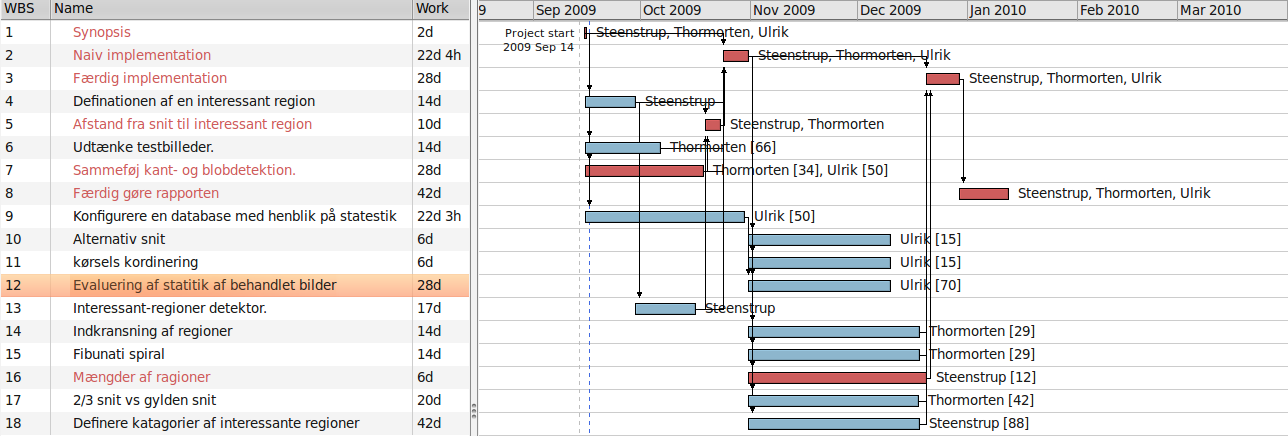
\includegraphics[angle=90, scale=0.45]{pictures/tidsplan.png}
\end{center}


\section*{Tekniske detaljer}
Vi har valgt at udvikle vores implementation i Python. Valget begrunder
sig hovedsageligt i at Python er et godt værktøj til at lave prototyper
i. Vi undgår herved at bruge alt for meget tid på at definere diverse
datastrukturer, fremfor at koncentrere os om kernen i projektet. Det der
kan argumentere imod valget af Python er at det kan være langsomt. Vores
vurdering er dog at dette ikke vil blive et problem, samt at vi i første
omgang ikke går efter at lave en hurtigt implementation, blot en
implementation der virker.

Til at udføre billedmanipulation benytter vi os af et bibliotek skrevet i C der
hedder OpenCV. Biblioteket er udviklet af Intel og tilbyder, udover et solidt
udvalg af algoritmer, bindinger til Python. Endelig er det meget
veldokumenteret og giver referencer til publikationer om bibliotekets
algoritmer. Biblioteket er udviklet med specielt henblik på real-tids
behandling af billeder, f.eks. med et videokamera som kilde, men egner sig også
til brug på enkelte billeder.

Vi ønsker at opbevare resultater fra kørsler i en database. Et endeligt
valg er ikke taget endnu, men vi vælger en let tilgængelig Open
Source-applikation, som let kan integreres med Pyhton, såsom MySQL eller
PostgreSQL.

Vores kode opbevares hos en gratis tjeneste i et git-repository. Koden
vil da til enhver tid kunne ses og hentes fra
\href{http://github.com/thorlund/gyldnesnit}{http://github.com/thorlund/gyldnesnit}.
Synopsis og rapport skrives i \LaTeX{} og kildekoden hertil vil også være
at finde i vores git-repository.


\section*{Disposition til rapport}
Vi forestiller os, at vores endelige rapport vil følge en disposition lignende
den nedenstående. Bemærk at underpunkterne ikke ligger helt fast, men alle
punkter på øverste niveau \emph{skal} være at finde i rapporten.

\begin{enumerate}
	\item Indledning
	\item Baggrund
		\begin{enumerate}
			\item Det Gyldne Snit
			\item Kunst og komposition
			\item Definition af det gyldne snit
		\end{enumerate}
	\item Vores implementering
		\begin{enumerate}
			\item Overblik
			\item Simpel algoritme
				\begin{enumerate}
					\item Intuitiv beskrivelse af tankerne bag algoritmen
				\end{enumerate}
			\item Kantdetektion
			\item Blobdetektion
		\end{enumerate}
	\item Vurdering
		\begin{enumerate}
			\item Afprøvning
			\item Resultater
			\item Optimeringer
		\end{enumerate}
	\item Litteratur
	\item Billag
		\begin{enumerate}
			\item Kildekode
			\item Malerier
		\end{enumerate}
\end{enumerate}


\section*{Relevant litteratur}
\begin{itemize}
	\item Study of 565 paintings - \href{http://arxiv.org/abs/physics/9908036/}{http://arxiv.org/abs/physics/9908036/}
\end{itemize}


%%%%%%%%%%%%%%%%%%%%%%%%%%%%%%%%%%%%%%%%%%%%%%%%%%%%%%%%%%%%%%%%%%%%%%%%%%%%%%%%%%%%%
% Litteratur
%%%%%%%%%%%%%%%%%%%%%%%%%%%%%%%%%%%%%%%%%%%%%%%%%%%%%%%%%%%%%%%%%%%%%%%%%%%%%%%%%%%%%

\newpage

\begin{thebibliography}{99}
%\addcontentsline{toc}{section}{Litteratur}

% Bog
%\bibitem[1]{AB0X} efternavn, fornavn, fornavn efternavn på andre forfattere: bogens titel, forlag, årstal
%\bibitem[1]{TMBC} Ægidius Mogensen, Torben: Basics of Compiler Design, - , 2007

% Artikel i tidsskrift
%\bibitem[2]{CD0X} efternavn, fornavn, fornavn efternavn på andre forfattere: titel, tidsskriftets navn, nr:sidetal, årstal
%\bibitem[2]{CD0X} efternavn, fornavn, fornavn efternavn på andre forfattere: titel, tidsskriftets navn, nr:sidetal, årstal
\bibitem[Dou]{Bib:Dou} S. Douady, Y. Couder: \href{http://www.math.ntnu.no/~jarlet/Douady96.pdf}{``Phyllotaxis as a Dynamical Self Organizing Process''}(PDF), Journal of Theoretical Biology, 178: 255–274, 1996,  doi:\href{http://dx.doi.org/10.1006\%2Fjtbi.1996.0026}{10.1006/jtbi.1996.0026}
\bibitem[WpC1]{Bib:WGold} Wikipedia contributors: ``Golden ratio'', Wikipedia, The Free Encyclopedia,\\
	\href{http://en.wikipedia.org/w/index.php?title=Golden\_ratio\&oldid=313121558}{http://en.wikipedia.org/w/index.php?title=Golden\_ratio\&oldid=313121558} (accessed September 11, 2009)
\bibitem[Wei]{Bib:MWGold} Weisstein, Eric W.: ``Golden Ratio.'', MathWorld -- A Wolfram Web Resource. \href{http://mathworld.wolfram.com/GoldenRatio.html}{http://mathworld.wolfram.com/GoldenRatio.html}
\bibitem[Knott]{Bib:Knott} Knott, Ron: ``Fibonacci Numbers and the Golden Section'', \href{http://www.mcs.surrey.ac.uk/Personal/R.Knott/Fibonacci/}{http://www.mcs.surrey.ac.uk/Personal/R.Knott/Fibonacci/}
\bibitem[Mark]{Bib:Mark} Markowsky, George: \href{http://www.umcs.maine.edu/~markov/GoldenRatio.pdf}{``Misconceptions about the Golden Ratio''}(PDF), College Mathematics Journal 23 (1): 2-19, 1992, doi:\href{http://dx.doi.org/10.2307\%2F2686193}{10.2307/2686193}
\bibitem[Ola]{Bib:Painting} Olariu, Agata: \href{http://arxiv.org/abs/physics/9908036/}{``Golden Section and the Art of Painting''}, 1999, \href{http://arxiv.org/pdf/physics/9908036v1}{http://arxiv.org/pdf/physics/9908036v1}(PDF)

% Konference
%\bibitem[3]{EF0X} efternavn, fornavn, fornavn efternavn på andre forfattere: titel, navn på konference, redaktører, forlag, land årstal

\end{thebibliography}

%\newpage
%\section*{Bilag} 
%\appendix

%\section{Source code}
%\input{materialer.tex}
%\newpage

\end{document}
